\documentclass[xcolor=table]{beamer}
\mode<presentation>
\usetheme{CambridgeUS}
\usepackage[english, russian]{babel}
\usepackage[utf8]{inputenc}
\usepackage[T2A]{fontenc}
\usepackage{sansmathaccent}
\usepackage{alltt}
\usepackage[table]{xcolor}
%\linespread{0.8}
\usepackage{minted}
%\usepackage{setspace}

\pdfmapfile{+sansmathaccent.map}
\title[Software Design]{Документация. Файлы. Модули. Пакеты}
\author{Наумов Д.А., доц. каф. КТ}
\date[22.11.2020] {Основы программной инженерии, 2020}

\begin{document}

%ТИТУЛЬНЫЙ СЛАЙД
\begin{frame}
  \titlepage
\end{frame}
  
%СОДЕРЖАНИЕ ЛЕКЦИИ
\begin{frame}
  \frametitle{Содержание лекции}
  \tableofcontents  
\end{frame}

\section{Документирование}

\begin{frame}{PEP8 - стиль кода в языке Python}
	Документирование кода в python -- достаточно важный аспект, ведь от нее порой зависит читаемость и быстрота понимания вашего кода, как другими людьми, так и вами через полгода.
	
	\medskip
	
	\textbf{PEP 257} описывает соглашения, связанные со строками документации \textit{python}, рассказывает о том, как нужно документировать python код.
	\begin{itemize}
		\item цель этого PEP -- стандартизировать структуру строк документации: что они должны в
себя включать, и как это написать (не касаясь вопроса синтаксиса строк документации).
		\item PEP описывает соглашения, а не правила или синтаксис.
		\item При нарушении этих соглашений, самое худшее, чего можно ожидать -- некоторых
неодобрительных взглядов. 
		\item Некоторые программы (например, docutils), знают о соглашениях.
	\end{itemize}	
\end{frame}

\begin{frame}{Строки документации}
	\textbf{Строки документации} -- строковые литералы, которые являются первым оператором в модуле, функции, классе или определении метода. 
	
	\medskip
		
	Такая строка документации становится специальным атрибутом \_\_doc\_\_ этого объекта.
	
	\medskip
	
	\begin{itemize}
		\item Все модули должны, как правило, иметь строки документации, и все функции и классы,
экспортируемые модулем также должны иметь строки документации. 
		\item Публичные методы (в том числе \_\_init\_\_) также должны иметь строки документации. 
		\item Пакет модулей может быть документирован в \_\_init\_\_.py.
		\item Для согласованности, всегда используйте  \grqq\grqq\grqq double quotes\grqq\grqq\grqq для строк документации.
		\item Используйте r\grqq\grqq\grqq raw double quotes\grqq\grqq\grqq, если вы будете использовать обратную косую черту в строке документации.
	\end{itemize}	
\end{frame}

\begin{frame}[fragile]{Однострочные строки документации}
	\begin{minted}{python}
def kos_root():
	"""Return the pathname of the KOS root directory."""
	global _kos_root
	if _kos_root: 
		return _kos_root
	\end{minted}
	\begin{itemize}
		\item Используйте тройные кавычки, даже если документация умещается на одной строке. 
		\item Не добавляйте пустых строк перед или после документации.
	\end{itemize}
	
	\medskip
	
	Однострочная строка документации не должна быть <<подписью>> параметров функции /
метода:
	\begin{minted}{python}
def function(a, b):
	"""function(a, b) -> list"""
	\end{minted}
\end{frame}

\begin{frame}[fragile]{Многострочные строки документаци}
	Многострочные строки документации состоят из однострочной строки документации с
последующей пустой строкой, а затем более подробным описанием. 
	\begin{minted}{python}
def complex(real=0.0, imag=0.0):
	"""Form a complex number.
	
	Keyword arguments:
	real -- the real part (default 0.0)
	imag -- the imaginary part (default 0.0)
	"""

	if imag == 0.0 and real == 0.0: 
		return complex_zero
	\end{minted}
	Первая строка может быть использована автоматическими средствами индексации, поэтому важно, чтобы она находилась на одной строке и была отделена от остальной документации пустой строкой. 
\end{frame}

\begin{frame}[fragile]{Строки документации скрипта}
	\begin{itemize}
		\item должны быть доступны в качестве <<сообщения по использованию>>, напечатанной, когда программа вызывается с некорректными или отсутствующими аргументами (или, возможно, с опцией -h, для
помощи). 
		\item такая строка документации должна документировать функции программы и
синтаксис командной строки, переменные окружения и файлы. 
		\item сообщение по использованию может быть довольно сложным (несколько экранов) и должно быть достаточным для нового пользователя для использования программы должным образом, а также полный справочник со всеми вариантами и аргументами для искушенного пользователя. 
	\end{itemize}	
\end{frame}

\begin{frame}[fragile]{Строки документации модуля}
	Строки документации модуля должны, как правило, перечислять:
	\begin{itemize}
		\item классы, 
		\item исключения,
		\item функции (и любые другие объекты), 
	\end{itemize}	
	которые экспортируются модулем, с краткими пояснениями (в одну строчку) каждого из них. 
	
	\medskip
	
	Строки документации пакета модулей (т.е. строка документации в \_\_init\_\_.py) также должны включать модули и подпакеты.
\end{frame}

\begin{frame}[fragile]{Строки документации функции/метода}
	Строки документации функции или метода должны и документировать:
	\begin{itemize}
		\item аргументы, 
		\item возвращаемые значения
		\item побочные эффекты, 
		\item исключения, 
		\item дополнительные аргументы, 
		\item именованные аргументы, 
		\item ограничения на вызов функции.
	\end{itemize}
\end{frame}

\begin{frame}[fragile]{Строки документации класса}
	Строки документации класса обобщают его поведение и перечисляют:
	\begin{itemize}
		\item открытые методы 
		\item переменные экземпляра.
	\end{itemize}
	Если класс предназначен для подклассов, и имеет дополнительный интерфейс для подклассов, этот интерфейс должен быть указан отдельно (в строке документации). 

	\medskip

	Конструктор класса должен быть задокументирован в документации метода \_\_init\_\_. 
	
	\medskip
	
	Отдельные методы должны иметь свои строки документации.	
\end{frame}

\section{Аннотация типов}

\begin{frame}
  \frametitle{Содержание лекции}
  \tableofcontents[current]
\end{frame}

\begin{frame}[fragile]{Назначение аннотаций}
	Аннотации нужны для того чтобы повысить информативность исходного кода, и иметь возможность с помощью специальных инструментов производить его анализ. 

	\medskip
		
	Согласно PEP 3107 могут быть следующие варианты использования аннотаций:
	\begin{itemize}
		\item проверка типов;
		\item расширение функционала IDE в части предоставления информации об ожидаемых типах аргументов и типе возвращаемого значения у функций;
		\item перегрузка функций и работа с дженериками;
		\item взаимодействие с другими языками;
		\item использование в предикатных логических функциях;
		\item маппинг запросов в базах данных;
		\item маршалинг параметров в RPC (удаленный вызов процедур).
	\end{itemize}
\end{frame}

\begin{frame}[fragile]{Контроль типов}
	Один из возможных вариантов (наверное самый логичный) решения данной задачи -- это использование
комментариев, составленных определенным образом. 

	\begin{minted}{python}
	name = "John" # type: str
	\end{minted}
	
	Мы создали переменную с именем name и предполагаем, что ее тип - str. Естественно, для самого интерпретатора Python это не имеет значения, мы, без труда можем продолжить нашу мини программу таким образом:
	\begin{minted}{python}
	name = "John" # type: str
	print(name)
	name = 10
	print(name)	
	\end{minted}
	И это будет корректно с точки зрения Python.
\end{frame}

\begin{frame}[fragile]{Контроль типов}
	Один из возможных вариантов (наверное самый логичный) решения данной задачи -- это использование
комментариев, составленных определенным образом. 

	\begin{minted}{python}
	name = "John" # type: str
	\end{minted}
	
	Мы создали переменную с именем name и предполагаем, что ее тип - str. Естественно, для самого интерпретатора Python это не имеет значения, мы, без труда можем продолжить нашу мини программу таким образом:
	\begin{minted}{python}
	name = "John" # type: str
	print(name)
	name = 10
	print(name)	
	\end{minted}
	И это будет корректно с точки зрения Python.
\end{frame}

\begin{frame}[fragile]{Контроль типов}
	Если необходимо проконтролировать, что переменной name будут присваиваться значения только строкового типа, мы должны: 
	\begin{enumerate}
		\item указать в комментарии о нашем намерение
		\item использовать специальный инструмент, который выполнит соответствующую проверку.	
	\end{enumerate}

	Установка модуля с помощью pip:
	\begin{minted}{bash}
	python -m pip install mypy
	\end{minted}
	
	Если мы сохраним приведенный выше код в файле type\_tester.py и выполним следующую команду:

	\begin{minted}{bash}
	python -m mypy test_type.py
	\end{minted}
	Получим такое сообщение:
	\begin{minted}{bash}
test_type.py:3: error: Incompatible types in assignment
(expression has type "int", variable has type "str")
	\end{minted}
	Оно говорит о том, что обнаружено несоответствие типов в операции присваивание: переменная имеет тип str, а ей присвоено значение типа int.
\end{frame}

\begin{frame}[fragile]{ Обзор PEP’ов регламентирующий работу с аннотациями}
	Работу с аннотациями регламентируют четыре ключевых документа: 
	\begin{enumerate}
		\item PEP 3107 — Function Annotations
		\begin{itemize}
			\item описывается синтаксис использования аннотаций в функциях Python
			\item аннотации не имеют никакого семантического значения для интерпретатора Python и предназначены только для анализа сторонними приложениями
			\item аннотировать можно аргументы функции и возвращаемое ей значение.
		\end{itemize}
		\item PEP 484 — Type Hints
		\item PEP 526 — Syntax for Variable Annotations
		\item PEP 563 — Postponed Evaluation of Annotations
	\end{enumerate}
\end{frame}

\begin{frame}[fragile]{ Обзор PEP’ов регламентирующий работу с аннотациями}
	Работу с аннотациями регламентируют четыре ключевых документа: 
	\begin{enumerate}
		\item PEP 3107 — Function Annotations
		\item PEP 484 — Type Hints
		\begin{itemize}
			\item представлены рекомендации по использованию аннотаций типов
			\item аннотация типов упрощает статический анализ кода, рефакторинг, контроль типов в рантайме и кодогенерацию, использующую информацию о типах
			\item определены следующие варианты работы с аннотациями:
			\begin{itemize}
				\item использование аннотаций в функциях согласно PEP 3107, 
				\item аннотация типов переменных через комментарии в формате \# type: type\_name
				\item использование stub-файлов.			
			\end{itemize}
		\end{itemize}		
		\item PEP 526 — Syntax for Variable Annotations
		\item PEP 563 — Postponed Evaluation of Annotations
	\end{enumerate}
\end{frame}

\begin{frame}[fragile]{ Обзор PEP’ов регламентирующий работу с аннотациями}
	Работу с аннотациями регламентируют четыре ключевых документа: 
	\begin{enumerate}
		\item PEP 3107 — Function Annotations
		\item PEP 484 — Type Hints
		\item PEP 526 — Syntax for Variable Annotations
		\begin{itemize}
			\item приводится описание синтаксиса для аннотации типов переменных (базируется на PEP 484), использующего языковые конструкции, встроенные в Python.
		\end{itemize}				
		\item PEP 563 — Postponed Evaluation of Annotations
		\begin{itemize}
			\item предлагается использовать отложенную обработку аннотаций, это позволяет определять переменные до получения информации об их типах и ускоряет выполнение программы.
		\end{itemize}		
	\end{enumerate}
\end{frame}

\begin{frame}[fragile]{Использование аннотаций в функциях}
	В функциях мы можем аннотировать аргументы и возвращаемое значение.
	\begin{minted}{python}
def repeater(s: str, n: int) -> str:
	return s * n
	\end{minted}
	\begin{itemize}
		\item аннотация для аргумента определяется через двоеточие после его имени;
		\item аннотация, определяющая тип возвращаемого функцией значения, указывается после ее имени с использованием символов ->	;
		\item доступ к аннотациям функции можно получить через атрибут \_\_annotations\_\_; 
		\item аннотации представлены в виде словаря, где ключами являются атрибуты, а значениями - аннотации; 
		\item возвращаемое функцией значение хранится в записи с ключом return;
		\item для lambda-функций аннотации не поддерживаются.
	\end{itemize}
\end{frame}

\begin{frame}[fragile]{Создание аннотированных переменных}
	Можно использовать один из трех способов создания аннотированных переменных:
	\begin{minted}{python}
	var = value # type: annotation
	var: annotation; var = value
	var: annotation = value
	\end{minted}

	Рассмотрим это на примере работы со строковой переменной с именем name:
	\begin{minted}{python}
	name = 'John' # type: str
	name: str; name = 'John'
	name: str = 'John'
	\end{minted}
\end{frame}

\begin{frame}[fragile]{Создание аннотированных переменных}
	\begin{minted}{python}
	from typing import List, Tuple
	# список
	scores: List[int] = [1 ]
	# кортеж
	pack: Tuple[int, int, int] = (1 , 2, 3)
	# логическая переменная
	flag: bool
	flag = True
	# класс
	class Point:
		x: int
		y: int		
		def __init__(self, x: int, y: int):
			self.x = x
			self.y = y
	\end{minted}
\end{frame}

\begin{frame}[fragile]{Контроль типов с использованием аннотаций}
	Для проверки можно использовать уже знакомый нам инструмент mypy. Напишем вот такой код:
	\begin{minted}{python}
	a: int = 10
	b: int = 15	
	def sq_sum(v1: int, v2: int) -> int:
		return v1 ** 2 + v2 ** 2
	print(sq_sum(a, b))
	\end{minted}
	
	Сохраним его в файле с именем work.py и запустим mypy для анализа:
	> python -m mypy work.py
	
	Если не указывать дополнительные ключи, то окно консоли будет чистым, т. к. mypy не найдет никаких ошибок в вашем коде.
\end{frame}

\begin{frame}[fragile]{Контроль типов с использованием аннотаций}
	Но если заменить первую строку:
	\begin{minted}{python}
	а: int = 10
	\end{minted}
на такую:
	\begin{minted}{python}
	а: int = 10.3
	\end{minted}
	и вновь запустить mypy, то увидим вот такое сообщение:
	\begin{minted}{bash}
work.py:7: error: Argument 1 to 'sq_sum' has incompatible type 'float'; expected 'int'
	\end{minted}

	При этом, естественно, код будет выполняться без всяких проблем, потому что интерпретатор Python в данном случае не обращает внимание на аннотации.	
\end{frame}

\section{Работа с модулями}

\begin{frame}
  \frametitle{Содержание лекции}
  \tableofcontents[current]
\end{frame}

\begin{frame}[fragile]{Инструкция import}
	Модулем в Python называется любой файл с программой. 	

	\begin{itemize}
		\item Каждая программа может импортировать модуль и получить доступ к его классам, функциям и объектам. 	
		\item При импорте модуля происходит его выполнение (интерпретация).
	\end{itemize}	
	
	Подключить модуль можно с помощью инструкции \textbf{import}.
	\begin{minted}{python}
	import os
	os.getcwd()
	\end{minted}
	
	Одной инструкцией можно подключить несколько модулей, хотя этого не рекомендуется делать, так как это снижает читаемость кода. 
	\begin{minted}{python}
	import time, random
	print(time.time())
	print(random.random())
	\end{minted}
\end{frame}

\begin{frame}[fragile]
	После импортирования модуля его название становится переменной, через которую
можно получить доступ к атрибутам модуля. 	
	\begin{minted}{python}
	import math
	print(math.e)
	\end{minted}
	
	Если указанный атрибут модуля не будет найден, возбудится исключение AttributeError. А если не удастся найти модуль для импортирования, то ImportError. 
	\begin{minted}{python}
	import notexist
Traceback (most recent call last):
File "", line 1, in import notexist
ImportError: No module named 'notexist'
	import math
	print(math.Ё)
Traceback (most recent call last):
File "", line 1, in math.Ё
AttributeError: 'module' object has no attribute 'Ё'
	\end{minted}
\end{frame}

\begin{frame}[fragile]{Инструкция from}
	Подключить определенные атрибуты модуля можно с помощью инструкции from. Она
имеет несколько форматов: 	
	\begin{minted}{python}
from <Название модуля> import <Атрибут 1> [ as <Псевдоним 1> ], [<Атрибут 2> [ as <Псевдоним 2> ] ...]
from <Название модуля> import *
	\end{minted}
	
	Первый формат позволяет подключить из модуля только указанные вами атрибуты. Для длинных имен также можно назначить псевдоним, указав его после ключевого слова as.
	\begin{minted}{python}
from math import e, ceil as c
print(e)
print(c(4.6))
	\end{minted}
	
	Импортируемые атрибуты можно разместить на нескольких строках, если их много, для лучшей читаемости кода:	
	\begin{minted}{python}
from math import (sin, cos,
                  tan, atan)
	\end{minted}
\end{frame}

\begin{frame}[fragile]
	Второй формат инструкции from позволяет подключить (почти) все переменные из модуля: 	
	\begin{minted}{python}
	from sys import *
	print(version)
	\end{minted}
	
	Для длинных имен также можно назначить псевдоним, указав его после ключевого слова as.
	\begin{minted}{python}
	from math import e, ceil as c
	print(e)
	print(c(4.6))
	\end{minted}
	
	\begin{itemize}
		\item если в модуле определена переменная \_\_all\_\_, то будут подключены только атрибуты из этого списка. 
		\item если переменная \_\_all\_\_ не определена, то будут подключены все атрибуты, не начинающиеся с нижнего подчёркивания. 
		\item импортирование всех атрибутов из модуля может нарушить пространство имен главной программы.
	\end{itemize}
\end{frame}

\begin{frame}[fragile]{Создание своего модуля}
	Создадим файл mymodule.py, в которой определим какие-нибудь функции: 	
	\begin{minted}{python}
def hello():
	print('Hello, world!')

def fib(n):
	a = b = 1
	for i in range(n - 2):
		a, b = b, a + b
	return b
	\end{minted}
	
	Теперь в этой же папке создадим другой файл, например, main.py:
	\begin{minted}{python}
	import mymodule
	
	mymodule.hello()
	print(mymodule.fib(10))
	\end{minted}
\end{frame}

\begin{frame}[fragile]
	При импортировании модуля его код выполняется полностью, то есть, если программа что-то печатает, то при её импортировании это будет напечатано. Этого можно избежать, если проверять, запущен ли скрипт как программа, или импортирован.
	\begin{minted}{python}
def hello():
	print('Hello, world!')

def fib(n):
	a = b = 1
	for i in range(n - 2):
		a, b = b, a + b
	return b
	
if __name__ == "__main__":
	hello()
	for i in range(10):
		print(fib(i))
	\end{minted}
\end{frame}

\section{Работа с файлами}

\begin{frame}
  \frametitle{Содержание лекции}
  \tableofcontents[current]
\end{frame}

\begin{frame}[fragile]{Открытие файла}
	Прежде, чем работать с файлом, его надо открыть.
	\begin{minted}{python}
f = open('text.txt', 'r')
	\end{minted}
	
	У функции open много параметров, рассмотрим первые два:
	\begin{itemize}
		\item первый -- имя файла. Путь к файлу может быть относительным или абсолютным. 
		\item второй -- режим, в котором будет открыт файл.	
	\end{itemize}
	\begin{figure}[h]
		\centering
		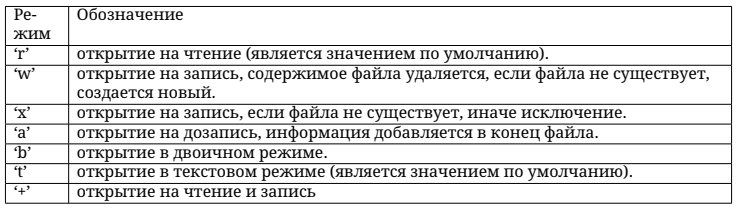
\includegraphics[scale=0.5]{images/lec11-pic01.png}
	\end{figure}	
\end{frame}

\begin{frame}[fragile]{Чтение из файла}
	Метод read читает весь файл целиком, если был вызван без аргументов, и n
символов, если был вызван с аргументом (целым числом n).
	\begin{minted}{python}
> f = open('text.txt')
> f.read(1)
'H'
> f.read()
'ello world!\nThe end.\n\n'
	\end{minted}
	
	Ещё один способ сделать это - прочитать файл построчно, воспользовавшись циклом for:
	\begin{minted}{python}
f = open('text.txt')
for line in f:
	line
	\end{minted}
\end{frame}

\begin{frame}[fragile]{Запись в файл}
	\begin{minted}{python}
> l = [str(i)+str(i-1) for i in range(20)]
> l
['0-1', '10', '21', '32', '43', '54', '65', '76', '87', '98', '109', 
'1110', '1211', '1312', '1413', '1514', '1615', '1716', '1817', '1918']
	\end{minted}
	
	Откроем файл на запись:
	\begin{minted}{python}
> f = open('text.txt', 'w')
	\end{minted}
	
	Запись в файл осуществляется с помощью метода write:
	\begin{minted}{python}
> for index in l:
	f.write(index + '\n')
4
3
3
3
3	
	\end{minted}
\end{frame}

\begin{frame}[fragile]{Запись в файл}
	\begin{minted}{python}
> l = [str(i)+str(i-1) for i in range(20)]
> l
['0-1', '10', '21', '32', '43', '54', '65', '76', '87', '98', '109', 
'1110', '1211', '1312', '1413', '1514', '1615', '1716', '1817', '1918']
	\end{minted}
	
	Откроем файл на запись:
	\begin{minted}{python}
> f = open('text.txt', 'w')
	\end{minted}
	
	Запись в файл осуществляется с помощью метода write:
	\begin{minted}{python}
> for index in l:
	f.write(index + '\n')
	\end{minted}
	
	После окончания работы с файлом его необходимо закрыть:	
	\begin{minted}{python}
> f.close()
	\end{minted}
\end{frame}

\begin{frame}[fragile]{Менеджеры контекста}
	Конструкция with ... as используется для оборачивания выполнения блока инструкций менеджером контекста. 		

	Синтаксис конструкции with:

	\begin{minted}{python}
with expression [as target] (, expression [as target])* :
	suite
	\end{minted}
	
	Выполнение менеджера контекста:
	\begin{enumerate}
\item Выполняется выражение в конструкции with ... as.
		\item Загружается специальный метод \_\_exit\_\_ для дальнейшего использования.
		\item Выполняется метод \_\_enter\_\_. Если конструкция with включает в себя слово as, то возвращаемое методом \_\_enter\_\_ значение записывается в переменную.
		\item Выполняется suite.
		\item Вызывается метод \_\_exit\_\_. В этот метод передаются параметры исключения, если оно произошло, или во всех аргументах значение None, если исключения не было.
	\end{enumerate}
\end{frame}

\begin{frame}[fragile]{Менеджеры контекста}
	Самый распространённый пример использования этой конструкции -- открытие файлов. Конструкция with гарантирует закрытие файла в любом случае:

	\begin{minted}{python}
with open('newfile.txt', 'w', encoding='utf-8') as g:
	d = int(input())
	print('1 / {} = {} '.format(d, 1 / d), file=g)
	\end{minted}
	
	Файл будет закрыт вне зависимости от того, что введёт пользователь.
\end{frame}

\end{document}